\documentclass[11pt]{article}
\usepackage[utf8]{inputenc}
\usepackage[T1]{fontenc} % uses T1 fonts (better quality)
\usepackage{lmodern} % uses Latin Modern fonts
\usepackage[margin=2cm]{geometry}
\usepackage[dvipsnames]{xcolor}
\usepackage{ragged2e}
\renewcommand{\baselinestretch}{1.15}
\usepackage{tikz}
\usetikzlibrary{automata,scopes,shapes,matrix,arrows,decorations.pathmorphing}
\tikzset{>={stealth}}
\usepackage{mathtools}
\usepackage{bm}
\usepackage{graphicx}
\usepackage[makeroom]{cancel}
\definecolor{OuterBlue}{HTML}{1370AA}
\definecolor{InnerBlue}{HTML}{9BC4DD}
\usepackage{pdfpages}
\usepackage{amssymb}
\usepackage{rotating}
% \definecolor{CrispBlue}{HTML}{0176AE}
% \colorlet{answer}{CrispBlue}
% \renewenvironment{center}{\par\centering\color{answer}}
% \renewenvironment{align*}{\color{answer}}

\begin{document}
\begin{center}
\LARGE{ECE 345 / ME 380: Introduction to Control Systems\\Problem Set \#3}\\[1.5em]
\large David Kirby\\[1.5em]
\large \textbf{Due Thursday, November 5, 2020 at 3:30pm}\\[2.5em]
\end{center}

% \noindent This homework is open note and open book. You are welcome to discuss the problems with other students, but your solutions and Matlab code \textit{must be written independently}. Copying will not tolerated.
\begin{enumerate}
    \item (+10 points) Consider a negative unity feedback system as in Figure 1 with \( G(s)=\displaystyle\frac{(s+1)(s+2)}{s^2(s^2 + 2s + 3)} \).
    \begin{figure}[h!]
    \centering
    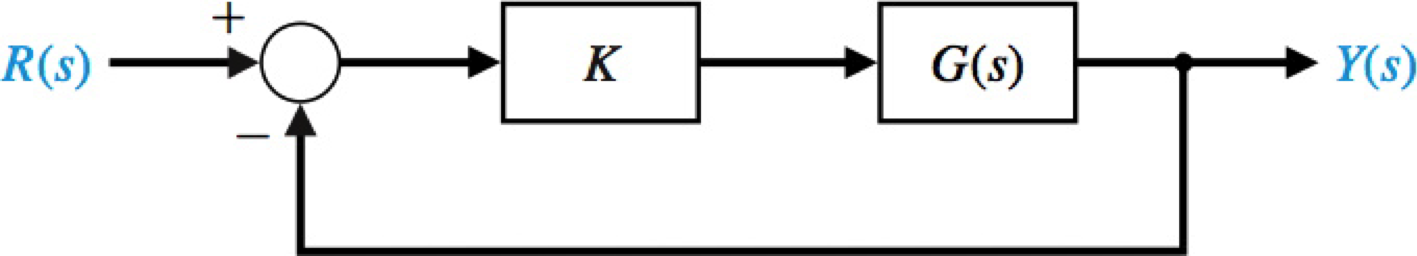
\includegraphics[width=0.55\textwidth]{./Images/Fig04-001.png}
    \caption{Negative unity feedback system.}
    \end{figure}
    \begin{enumerate}
        \item What is the type number of the closed-loop system \(\frac{Y(s)}{R(s)}\)?
        \begin{center}
            Type 2
        \end{center}
        \item What finite values of \(K\), if any, will yield a steady-state error less than or equal to 0.1, in response to a unit step input?
        \begin{align*}
            e_{ss} &=\frac{1}{1+K_p} &K_p &= \lim_{s \to 0}\ KG(s)\\
            &&&=\lim_{s \to 0}\ K\cdot \displaystyle\frac{(s+1)(s+2)}{s^2(s^2 + 2s + 3)}\\
            &&&=\infty\\
            e_{ss} &=0
        \end{align*}
        \begin{center}
            \(e_{ss}\) is 0, \(\ \therefore\ \) all values of \(K\) will meet this constraint.
        \end{center}
        \item What finite values of \(K\), if any, will yield a steady-state error less than or equal to 0.1, in response to a unit ramp input?
        \begin{align*}
            e_{ss} &=\frac{1}{K_v} &K_v &= \lim_{s \to 0}\ sKG(s)\\
            &&&=\lim_{s \to 0}\ s\cdot K\cdot \displaystyle\frac{(s+1)(s+2)}{s^2(s^2 + 2s + 3)}\\
            &&&=\infty\\
            e_{ss} &=0
        \end{align*}
        \begin{center}
            \(e_{ss}\) is 0, \(\ \therefore\ \) all values of \(K\) will meet this constraint.
        \end{center}
        \item What finite values of \(K\), if any, will yield a steady-state error less than or equal to 0.1, in response to a unit parabolic input?
        \begin{align*}
            e_{ss} &=\frac{1}{K_a} &K_a &= \lim_{s \to 0}\ s^2KG(s)\\
            &&&=\lim_{s \to 0}\ s^2 \cdot K\cdot \displaystyle\frac{(s+1)(s+2)}{s^2(s^2 + 2s + 3)}\\
            &&&=\frac{2K}{3}\\
            e_{ss} &=\frac{3}{2K}\leq 0.1\\ \\
            &K\geq 15
        \end{align*}

    \end{enumerate}
    \item (+15 points) Consider the following system, with reference input \(r(t)\) and disturbance input \(d(t)\).
    \begin{figure}[h!]
        \centering
        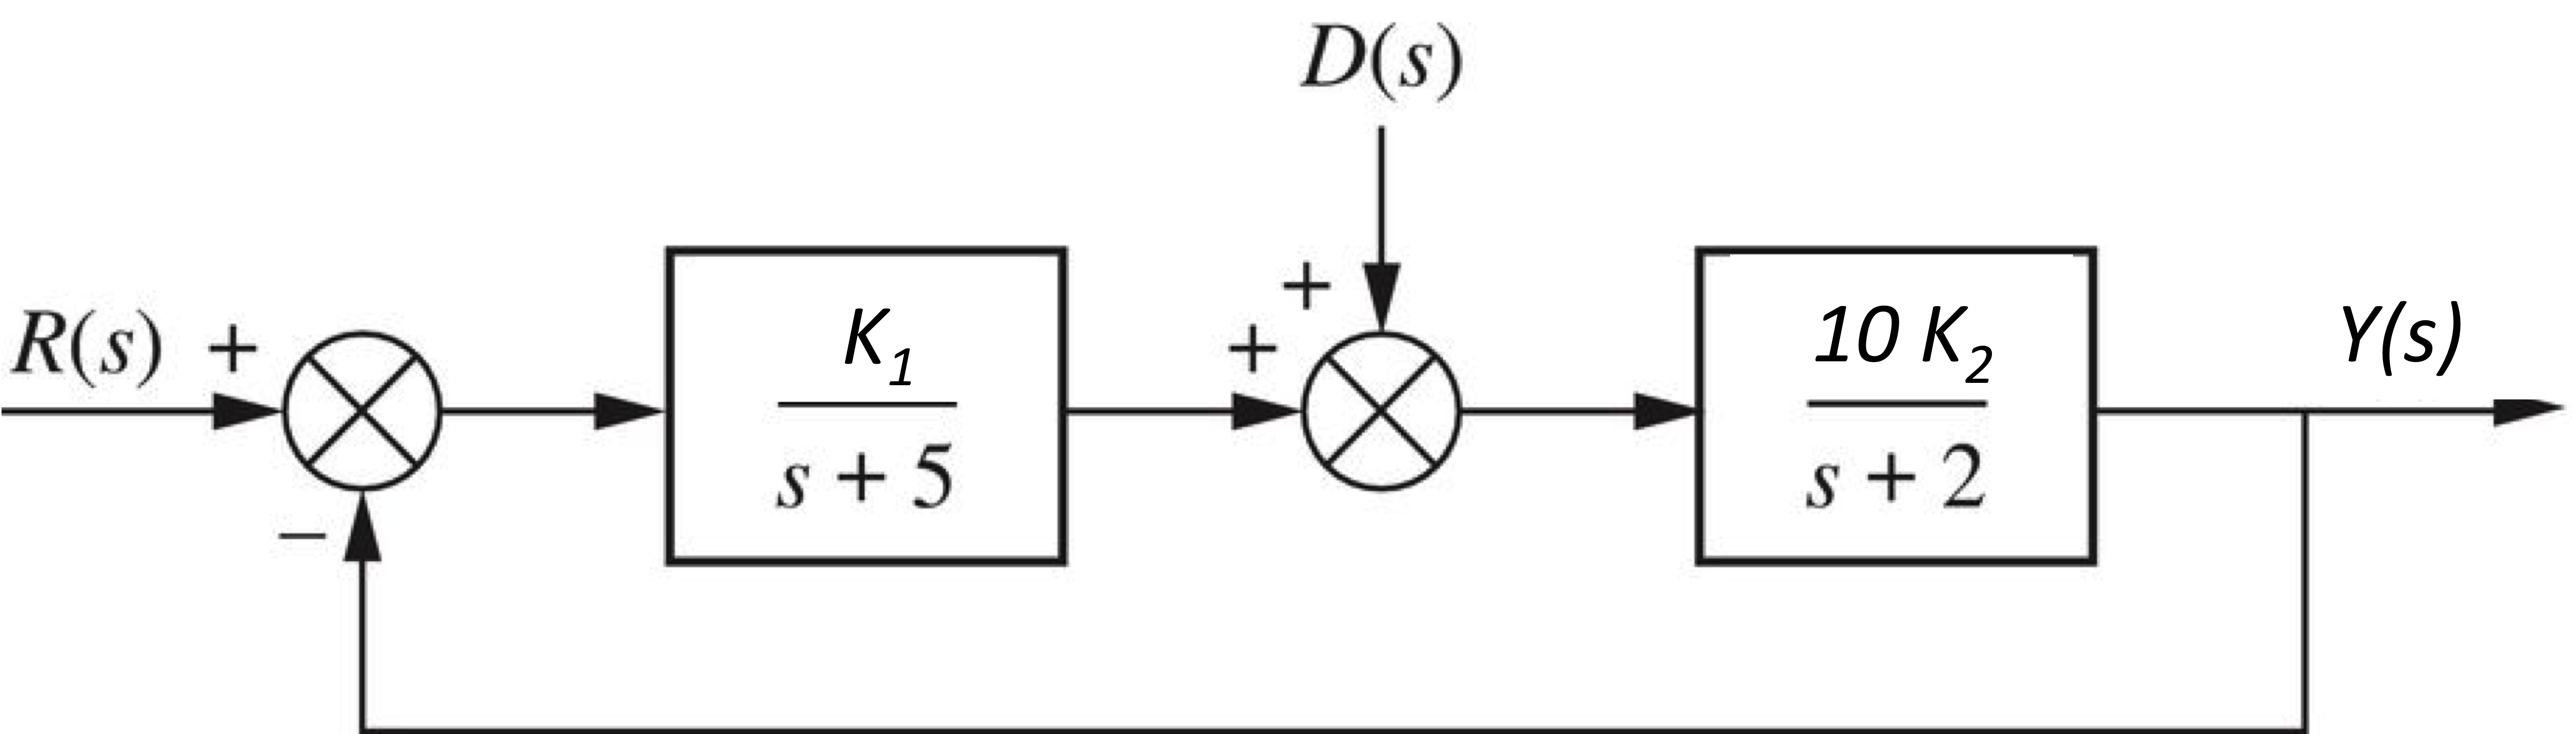
\includegraphics[width=0.55\textwidth]{./Images/Fig04-002.png}
        \end{figure}
    \begin{enumerate}
        \item Find the transfer function \(G_R(s)\) with output \(Y(s)\) and input \(R(s)\), and the transfer function \(G_D(s)\) with output \(Y(s)\) and input \(D(s)\), such that \(Y(s) = G_R(s)R(s)+G_D(s)D(s)\).
        \begin{center}
            Let \(\displaystyle G_1(s)=\frac{K_1}{s+5}\) (our controller) and \(\displaystyle G_2(s)=\frac{10K_2}{s+2}\) (our plant).
        \end{center}
        \begin{align*}
            G_R(s)&=\frac{G_1(s)G_2(s)}{1+G_1(s)G_2(s)} & G_D(s)&=\frac{G_2(s)}{1+G_1(s)G_2(s)}\\
            &=\frac{10K_1K_2}{(s+5)(s+2)+10K_1K_2}&&=\frac{10K_2(s+5)}{(s+5)(s+2)+10K_1K_2}\\
            &=\frac{10K_1K_2}{s^2+7s+10+10K_1K_2}&&=\frac{10K_2(s+5)}{s^2+7s+10+10K_1K_2}
        \end{align*}
        \item Describe the relationship between the characteristic equation of \(G_R(s)\) and the characteristic equation of \(G_D(s)\).
        \begin{center}
            The characteristic equations are the same: \(\Delta_R(s)=\Delta_D(s)\).
        \end{center}
        \item Do \(K_1 = 250\) and \(K_2 = \frac{1}{10}\) meet the following specifications? Why or why not?
        \begin{enumerate}
            \item The steady-state \textit{output response} due to a unit step disturbance input is 0.02.
            \begin{center}
                \( y_{ss} \leq 0.02 \) due to \( D(s)=\displaystyle\frac{1}{s} \) and pressure \(R(s)=0\).
            \end{center}
            \begin{align*}
                Y(s)&=\frac{10K_2(s+5)}{s^2+7s+10+10K_1K_2} \cdot D(s)\\
                &=\frac{s+5}{s^2+7s+260}\cdot \frac{1}{s}
            \end{align*}
            \begin{align*}
                \begin{turn}{15} \text{F.V.T.}
                \end{turn}\\
                y_{ss}&=\lim_{s \to 0}sY(s)\\
                &=\lim_{s \to 0}s\left( \frac{s+5}{s^2+7s+260}\cdot \frac{1}{s} \right)\\
                &=\frac{1}{52}=0.01923 \leq 0.02\ \checkmark
            \end{align*}
            \item The steady-state \textit{error} due to a unit step reference input is 0.05.
            \begin{center}
                \( e_{ss} \leq 0.05 \) for \( R(s)=\displaystyle\frac{1}{s} \) and pressure \(D(s)=0\).
            \end{center}
            \begin{align*}
                \frac{Y(s)}{R(s)}&=\frac{10K_1K_2}{(s+5)(s+2)+10K_1K_2}&\text{Type 0 system}
            \end{align*}
            \begin{align*}
                e_{ss} &=\frac{1}{1+K_p} &K_p &= \lim_{s \to 0}\ KG(s)\\
                &&&=\lim_{s \to 0}\ G_1(s)G_2(s)\\
                &&&=\lim_{s \to 0}\ \left( \frac{K_1}{s+5} \right) \left( \frac{10K_2}{s+2} \right)\\
                &&&=K_1K_2\\
                &&&=25\\
                e_{ss} &=\frac{1}{26} =0.03846 \leq 0.05\ \checkmark
            \end{align*}
            \begin{center}
                Yes, these values of \(K_1\ \&\ K_2\) meet the specifications.
            \end{center}
        \end{enumerate}
    \end{enumerate}
    \item (+15 points) Pulp dilution is an important part of the paper-making process. We model the dynamics of pulp dilution with plant \( G(s)=\displaystyle\frac{s+2}{s^2 + 2s + 3} \).
        \begin{figure}[h!]
        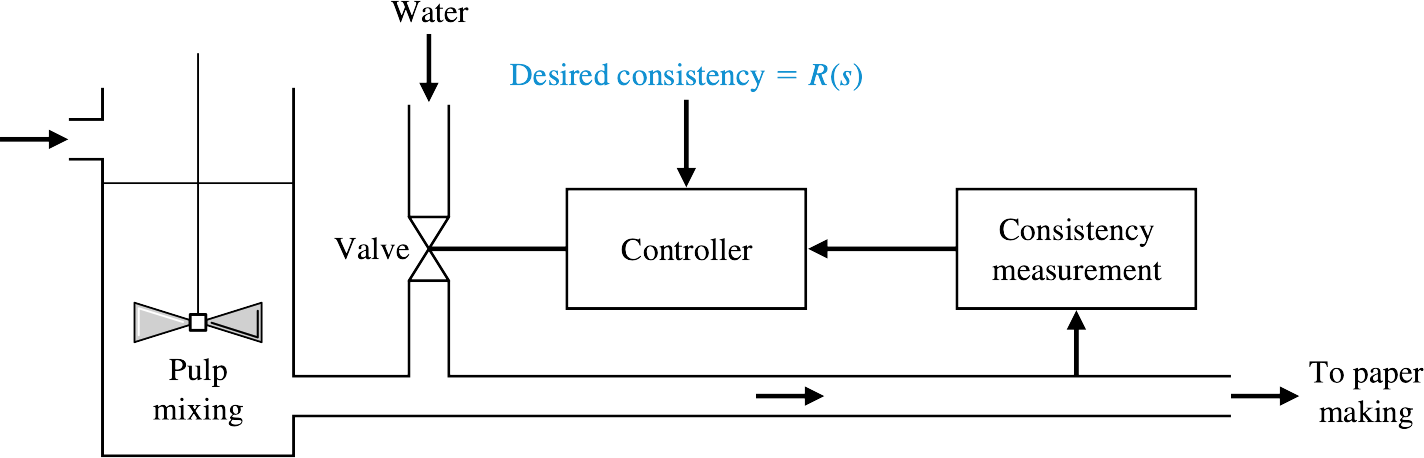
\includegraphics[width=0.5\textwidth]{./Images/Fig04-003.png}
        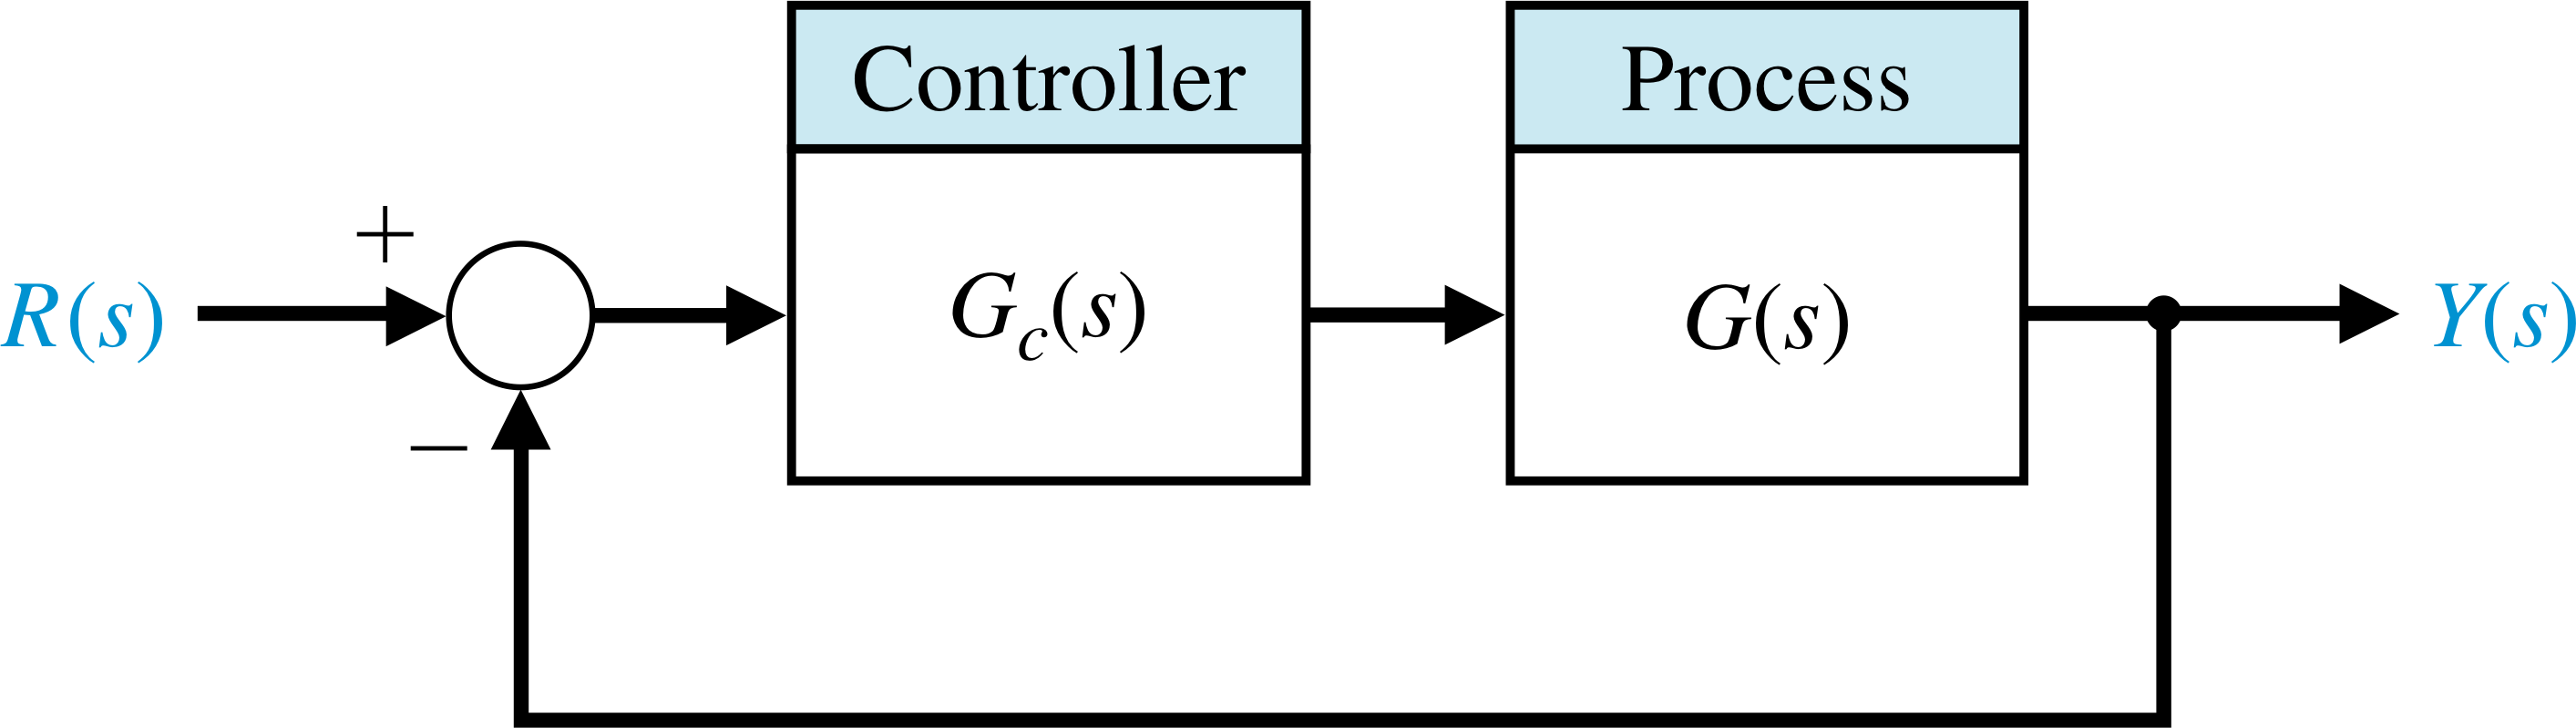
\includegraphics[width=0.5\textwidth]{./Images/Fig04-004.png}
        \end{figure}
        \begin{enumerate}
            \item Consider the controller \( G_c(s) = \displaystyle \frac{K}{s+1} \). What is the type number of the closed-loop system \(\frac{Y(s)}{R(s)}\)?
            \begin{center}
                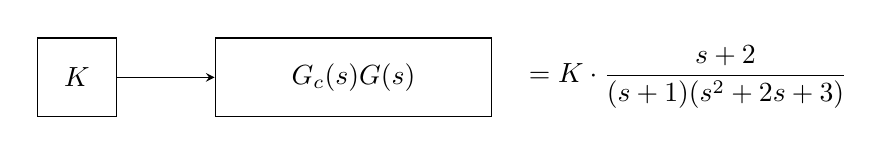
\begin{tikzpicture}
                    \matrix[column sep=0cm]{
                        \draw(0,0)rectangle (1,1);
                        \draw[->](1,0.5)--(2.25,0.5);
                        \node at (0.5,0.5) {$K$};
                    &
                        \draw(0,0)rectangle (3.5,1);
                        \node at (1.75,0.5) {$G_c(s)G(s)$};
                        \node at (6,0.5) {$=K \cdot\displaystyle\frac{s+2}{(s+1)(s^2 + 2s + 3)}$};
                        \\
                    };
                \end{tikzpicture}
                \\Type 0
            \end{center}\newpage
            \item What value of \( K > 0 \) will ensure that the steady-state error in response to a unit step input is at most 0.01?
            \begin{align*}
                e_{ss} &=\frac{1}{1+K_p} &K_p &= \lim_{s \to 0}\ KG(s)\\
                &&&=\lim_{s \to 0}\ K\cdot G_c(s)G(s)\\
                &&&=\lim_{s \to 0}\ K\cdot \frac{s+2}{(s+1)(s^2+2s+3)}\\
                &&&=\frac{2K}{3}\\
                e_{ss} &=\frac{1}{1+\displaystyle\frac{2K}{3}}\leq 0.01\\ \\
                &K\geq 148.5
            \end{align*}
            \item Now consider the controller \( G_c(s) = \displaystyle \frac{K}{s(s+1)} \). What is the type number of the closed-loop system \(\frac{Y(s)}{R(s)}\)?
            \begin{center}
                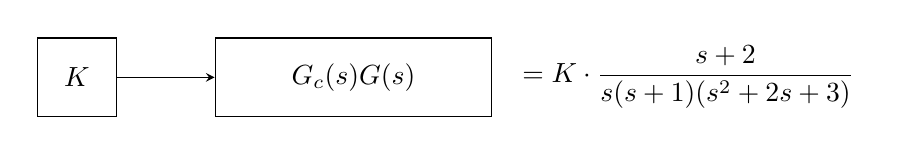
\begin{tikzpicture}
                    \matrix[column sep=0cm]{
                        \draw(0,0)rectangle (1,1);
                        \draw[->](1,0.5)--(2.25,0.5);
                        \node at (0.5,0.5) {$K$};
                    &
                        \draw(0,0)rectangle (3.5,1);
                        \node at (1.75,0.5) {$G_c(s)G(s)$};
                        \node at (6,0.5) {$=K \cdot\displaystyle\frac{s+2}{s(s+1)(s^2 + 2s + 3)}$};
                        \\
                    };
                \end{tikzpicture}
                \\Type 1
            \end{center}
            \item What value of \( K > 0 \) will ensure that the steady-state error in response to a unit step input is at most 0.01?
            \begin{align*}
                e_{ss} &=\frac{1}{1+K_p} &K_p &= \lim_{s \to 0}\ KG(s)\\
                &&&=\lim_{s \to 0}\ K\cdot G_c(s)G(s)\\
                &&&=\lim_{s \to 0}\ K\cdot \frac{s+2}{s(s+1)(s^2+2s+3)}\\
                &&&=\infty\\
                e_{ss} &=0
            \end{align*}
            \begin{center}
                \(e_{ss}\) is 0, \(\ \therefore\ \) all values of \(K\) will meet this constraint.
            \end{center}
            \item Consider the gain \( K = 150 \). Which controller has the best steady-state performance? Why?
            \begin{center}
                The controller with the extra \(s\) term (Type 1) will have the better steady-state performance. Even though \( K = 150 \) satisfies the constraint for the Type 0 system, there will still be slight steady-state error. The steady-state error for the Type 1 controller however will always be 0.
            \end{center}
        \end{enumerate}
\end{enumerate}
\end{document}